\section[3]{Our Adaptive SPS}

\begin{frame}{Our Adaptive SPS}
	\begin{exampleblock}{Our Proposal}
		An adaptive SPS based on \textbf{MAPE model} whose aim is to \textbf{adapt the number of replicas} of the operators according to the peaks in the data stream.
	\end{exampleblock}
	
	\only<1>{
	\begin{figure}
		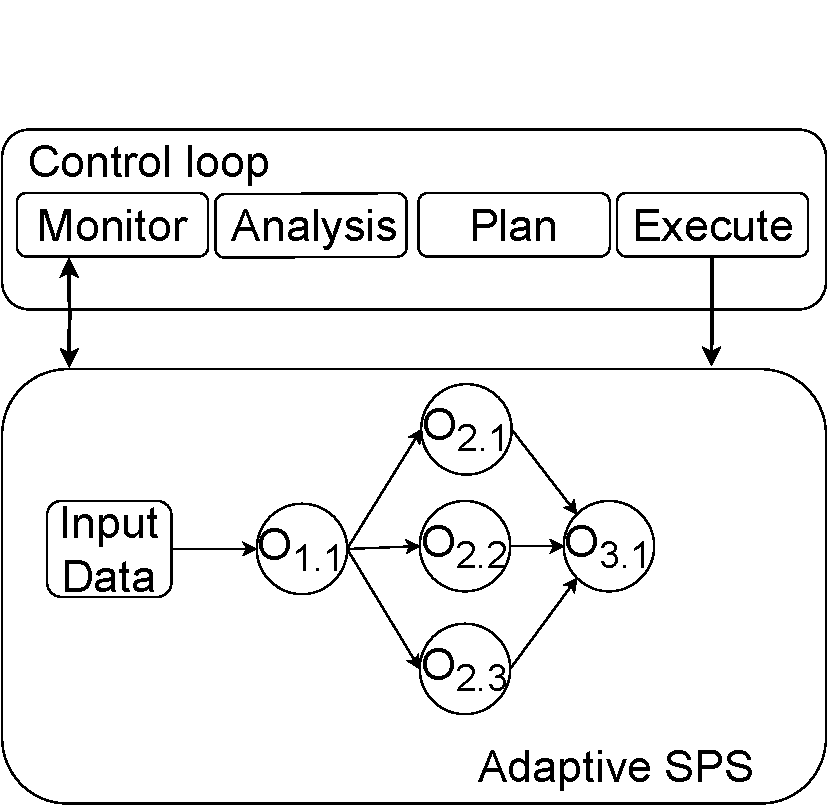
\includegraphics[scale=0.35]{images/problems/SPS-MAPE.pdf}
	\end{figure}
	}
	
	\only<2>{
	\begin{figure}
		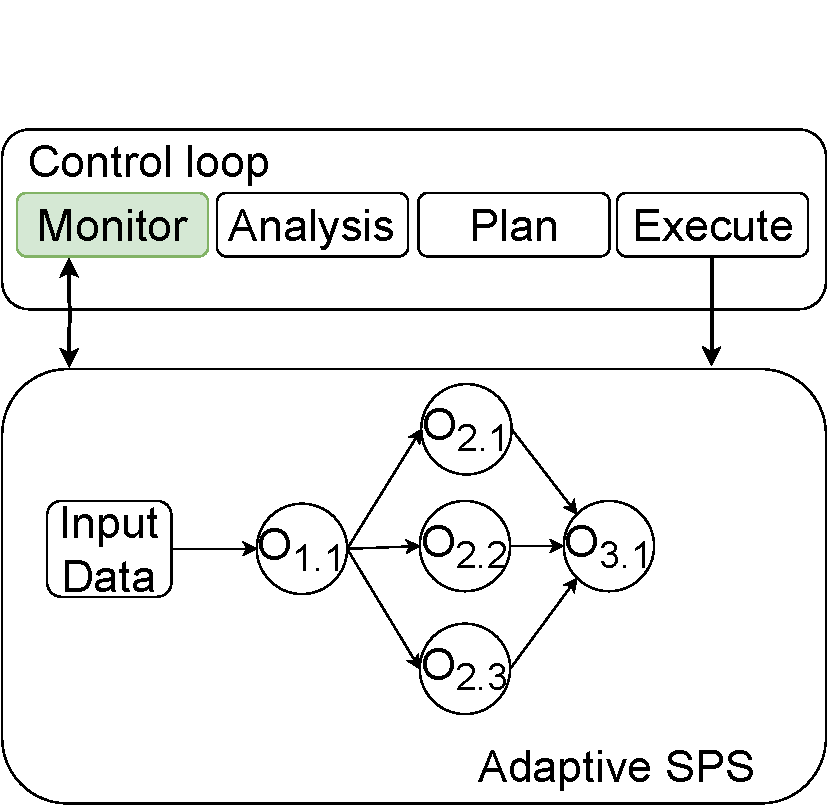
\includegraphics[scale=0.35]{images/problems/SPS-MAPE-M.pdf}
	\end{figure}
	}
	
	\only<3>{
	\begin{figure}
		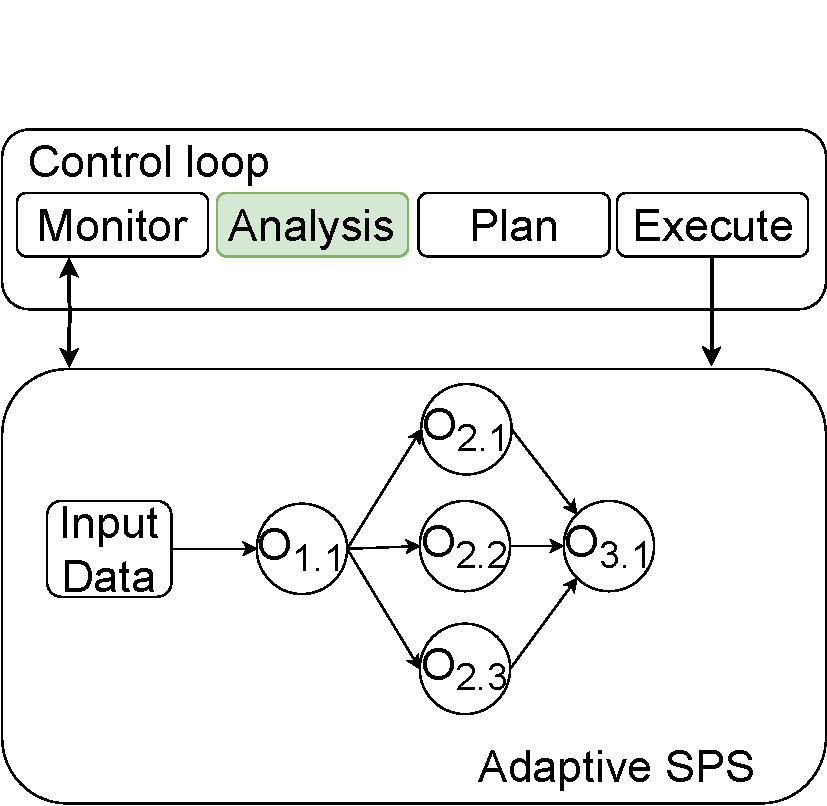
\includegraphics[scale=0.35]{images/problems/SPS-MAPE-A.pdf}
	\end{figure}
	}
	
	\only<4>{
	\begin{figure}
		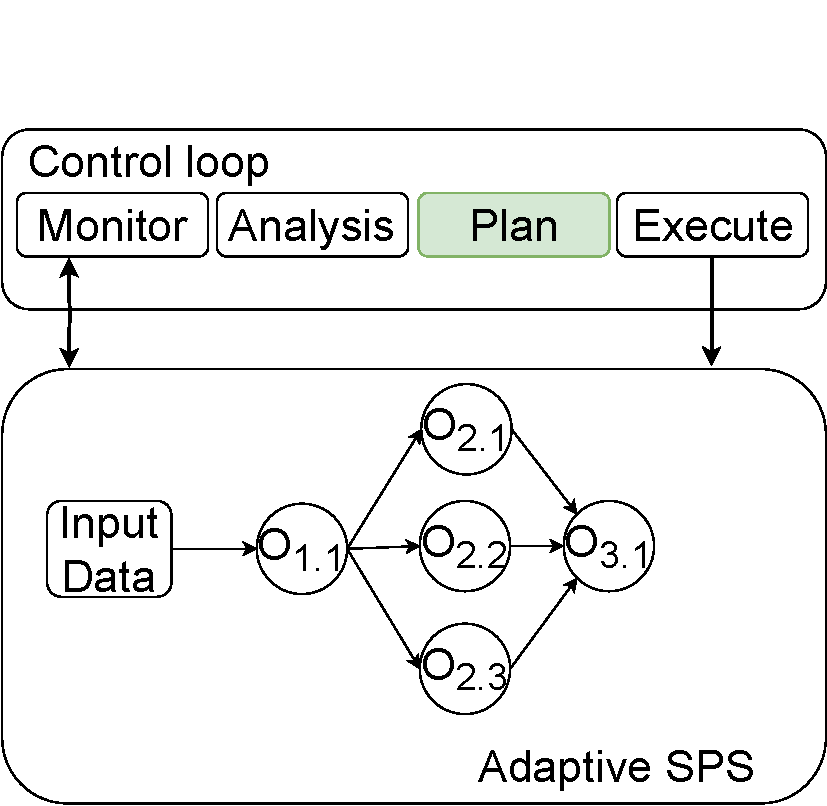
\includegraphics[scale=0.35]{images/problems/SPS-MAPE-P.pdf}
	\end{figure}
	}
	
	\only<5>{
	\begin{figure}
		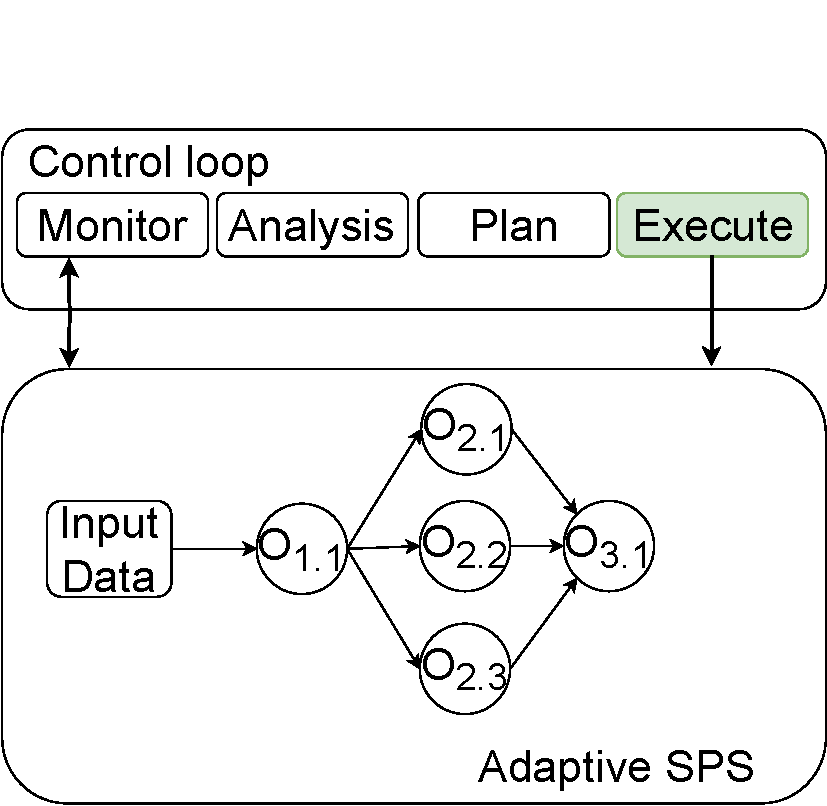
\includegraphics[scale=0.35]{images/problems/SPS-MAPE-E.pdf}
	\end{figure}
	}
\end{frame}

\begin{frame}{Our Adaptive SPS}
	Present two approaches:
	\begin{itemize}
		\item \textbf{Reactive approach} (RA-SPS): on-the-fly analysis of operator load
		\item \textbf{Predictive approach} (PA-SPS): predicting the number of replicas required
	\end{itemize}
\end{frame}

\begin{frame}{Our Adaptive SPS : Implementation}	
	An extension of Apache Storm	
		
	\begin{figure}
		
\includegraphics[scale=0.15]{images/concepts/Storm.png}
	\end{figure}
\end{frame}	

\begin{frame}{Storm limitation}	
	\begin{alertblock}{Limitation}
		Downtime in each reconfiguration	
	\end{alertblock}
	
	\begin{figure}
		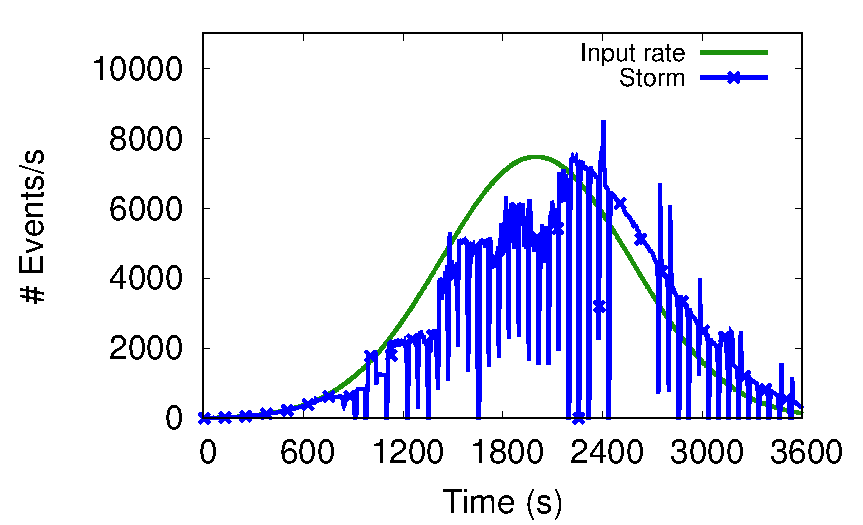
\includegraphics[scale=0.5]{images/problems/Pool.pdf}
	\end{figure}	
\end{frame}

\begin{frame}{Our Adaptive SPS : Pool of replicas}
	Pool of pre-allocate replicas for each operator.
	
	\only<1>{
	\begin{figure}
		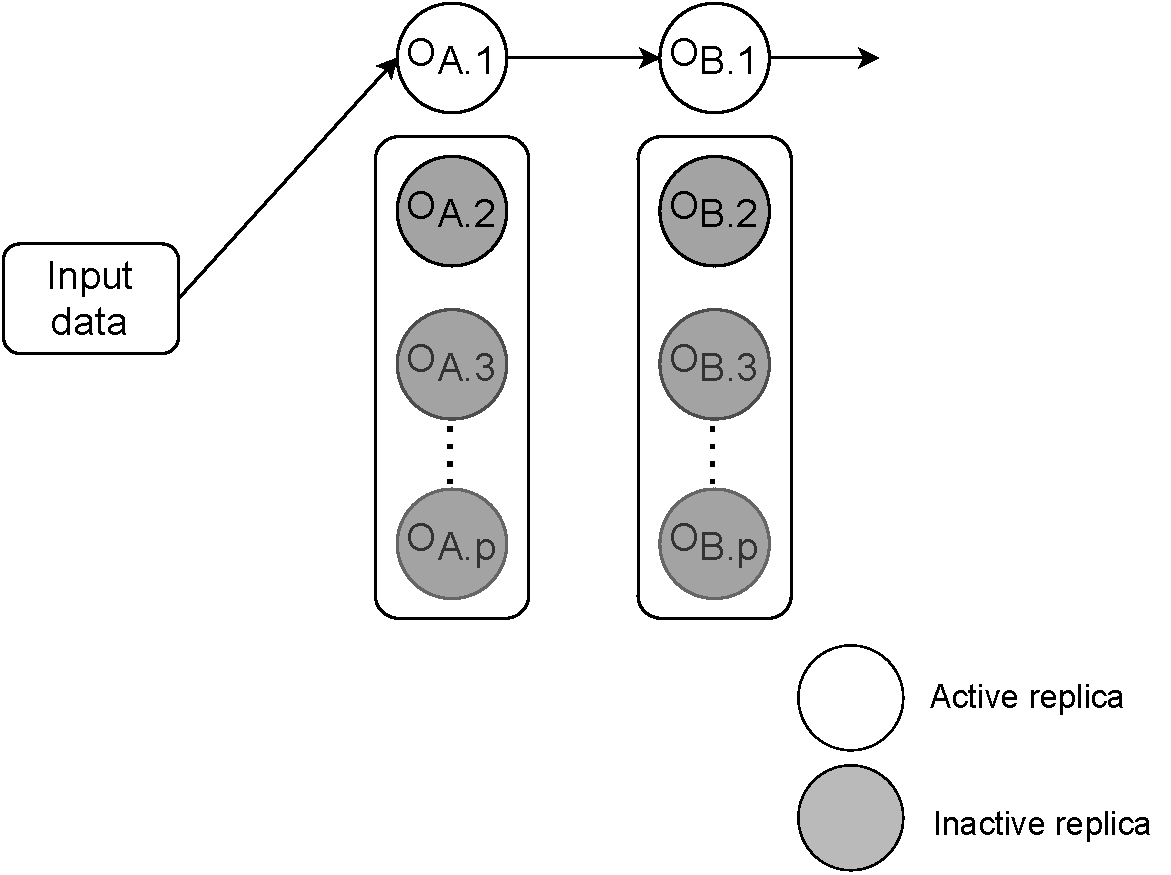
\includegraphics[width=0.75\textwidth]{images/problems/PoolReplicas1.pdf}
	\end{figure}
	}

	\only<2>{
	\begin{figure}
		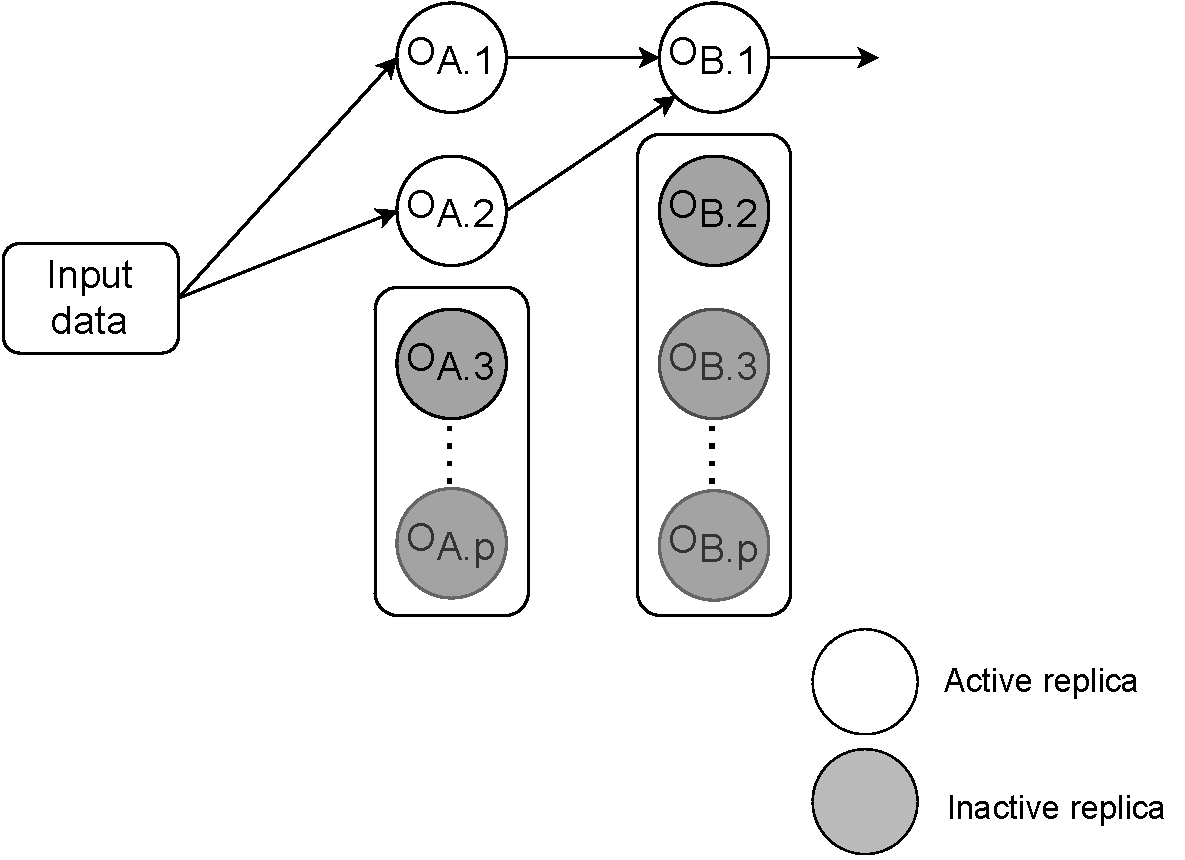
\includegraphics[width=0.75\textwidth]{images/problems/PoolReplicas2.pdf}
	\end{figure}
	}
\end{frame}

\begin{frame}{Storm limitation}
	
	\only<1>{
		Shuffle grouping (Round-robin) among the active replicas of an operator
	\begin{figure}
		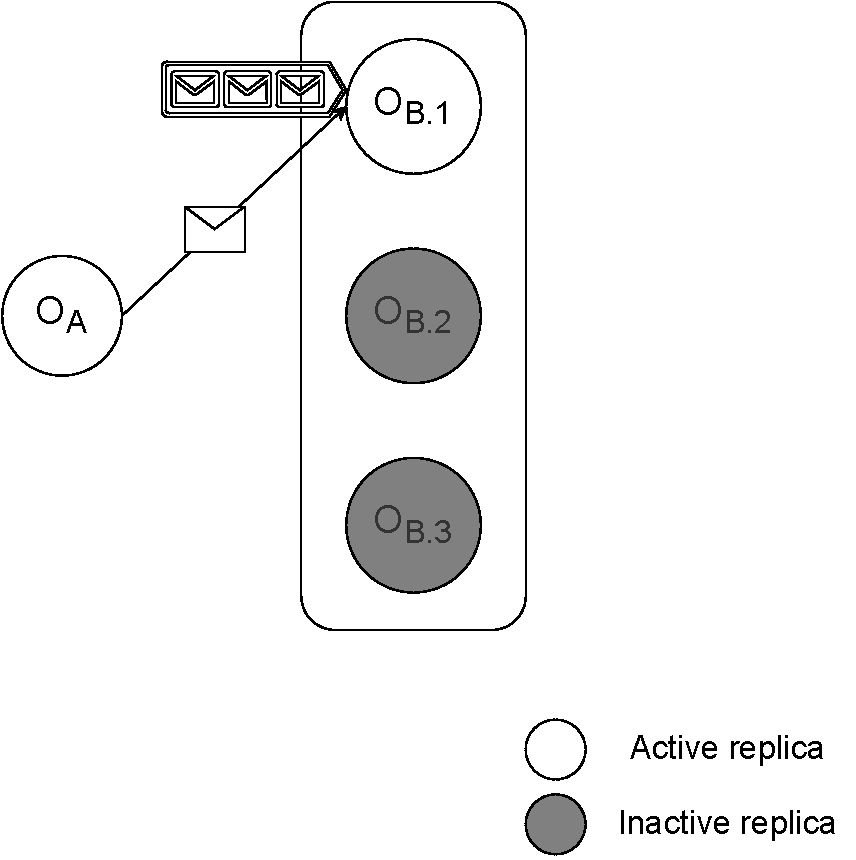
\includegraphics[width=0.62\textwidth]{images/problems/LoadGrouping.pdf}
	\end{figure}
	}

	\only<2>{
	\begin{alertblock}{Limitation}
		Load balancing among active replicas
	\end{alertblock}	
	
	\begin{figure}
		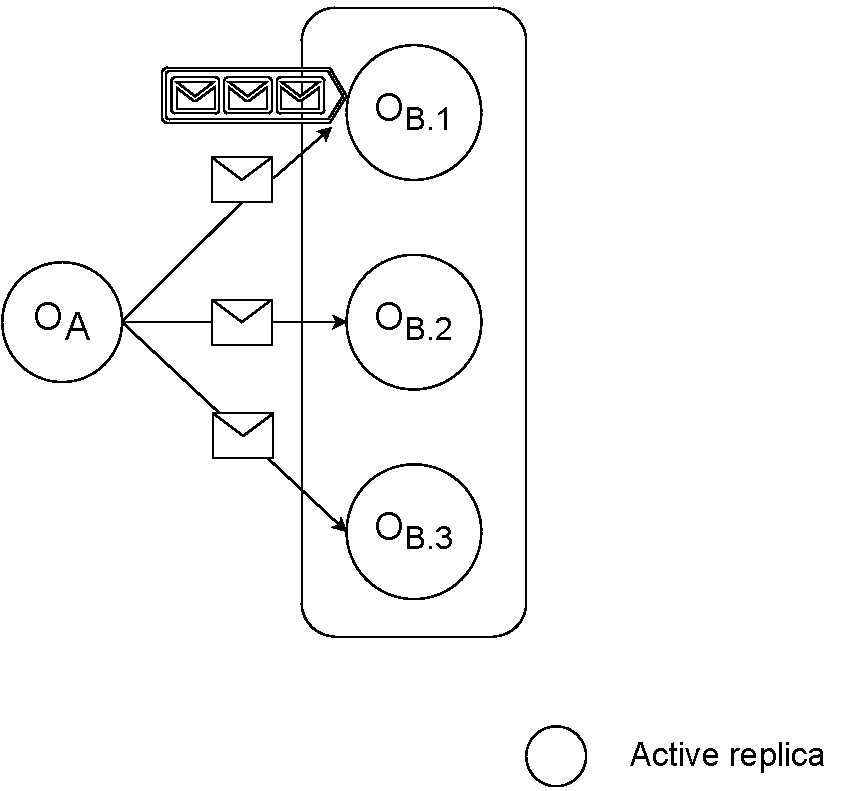
\includegraphics[width=0.64\textwidth]{images/problems/LoadGrouping1.pdf}
	\end{figure}
	}
\end{frame}
	
\begin{frame}{Our Adaptive SPS : Load-Aware grouping}
	Stream grouping for distributing the load among the active replicas of an operator
	\begin{figure}
		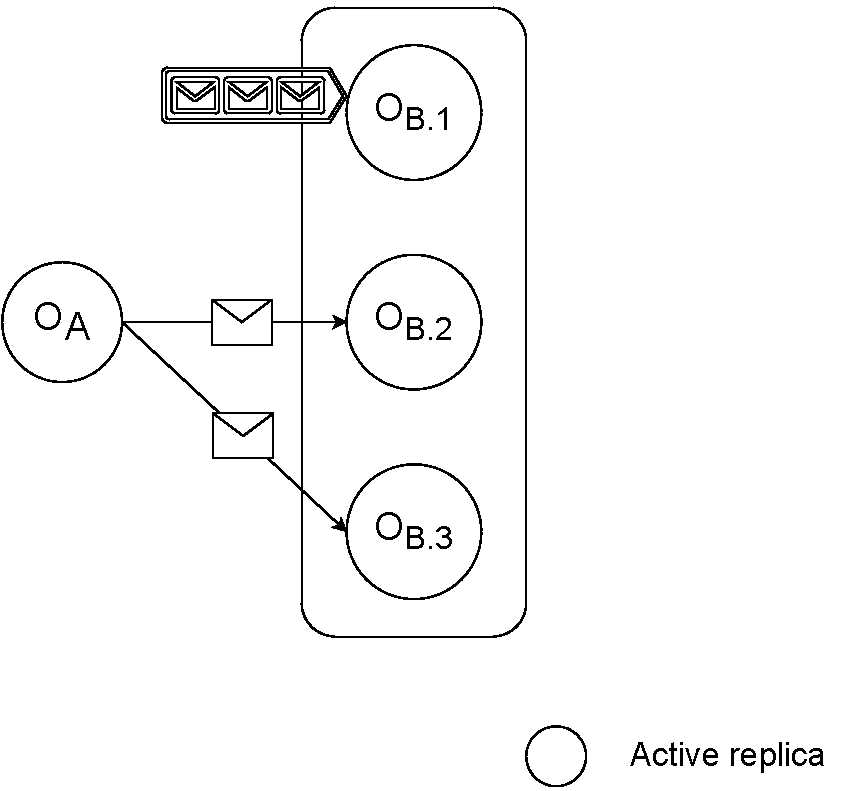
\includegraphics[width=0.65\textwidth]{images/problems/LoadGrouping2.pdf}
	\end{figure}
\end{frame}





